%!TEX root = ../article.tex

% Solution
\section{Solution}
\label{sec:solution}
Usually, provisioning the components of a smart place application is an operation
that is manually executed and requires expertise since that the software components must
be correctly installed and configured. Furthermore, every time that a new smart place is deployed
these operations must be repeated. With that in mind, in order to make the deployment of
smart places more efficient in Section~\ref{subs:sol_provisioning} we propose a solution
that automates the provision of smart places application in the cloud.

In the present work our main goal is to determine if a cloud-based deployment can meet the
requirements of RFID-based smart place applications, as mentioned in Section~\ref{sub:objectives}.
To achieve our goals we will follow two approaches to deploy the smart warehouse application: cloud
and fog. In Section~\ref{sub:sol_smart_warehouse_deployment}, we describe the alternative
architectures of the smart warehouse deployment.

% Provisioning
\subsection{Smart Place Provisioning}
\label{subs:sol_provisioning}
In this section we propose a mechanism that automates the provisioning of software for smart warehouse
applications in the cloud. Our solution relies on \acrfull{CM} tools that leverage existing software
stacks. Figure~\ref{fig:provisioning_generic_architecture} presents the architecture for the proposed
mechanism.

% Provisioning mechanism conceptual architecture
\begin{figure}[ht!]
  \centering
  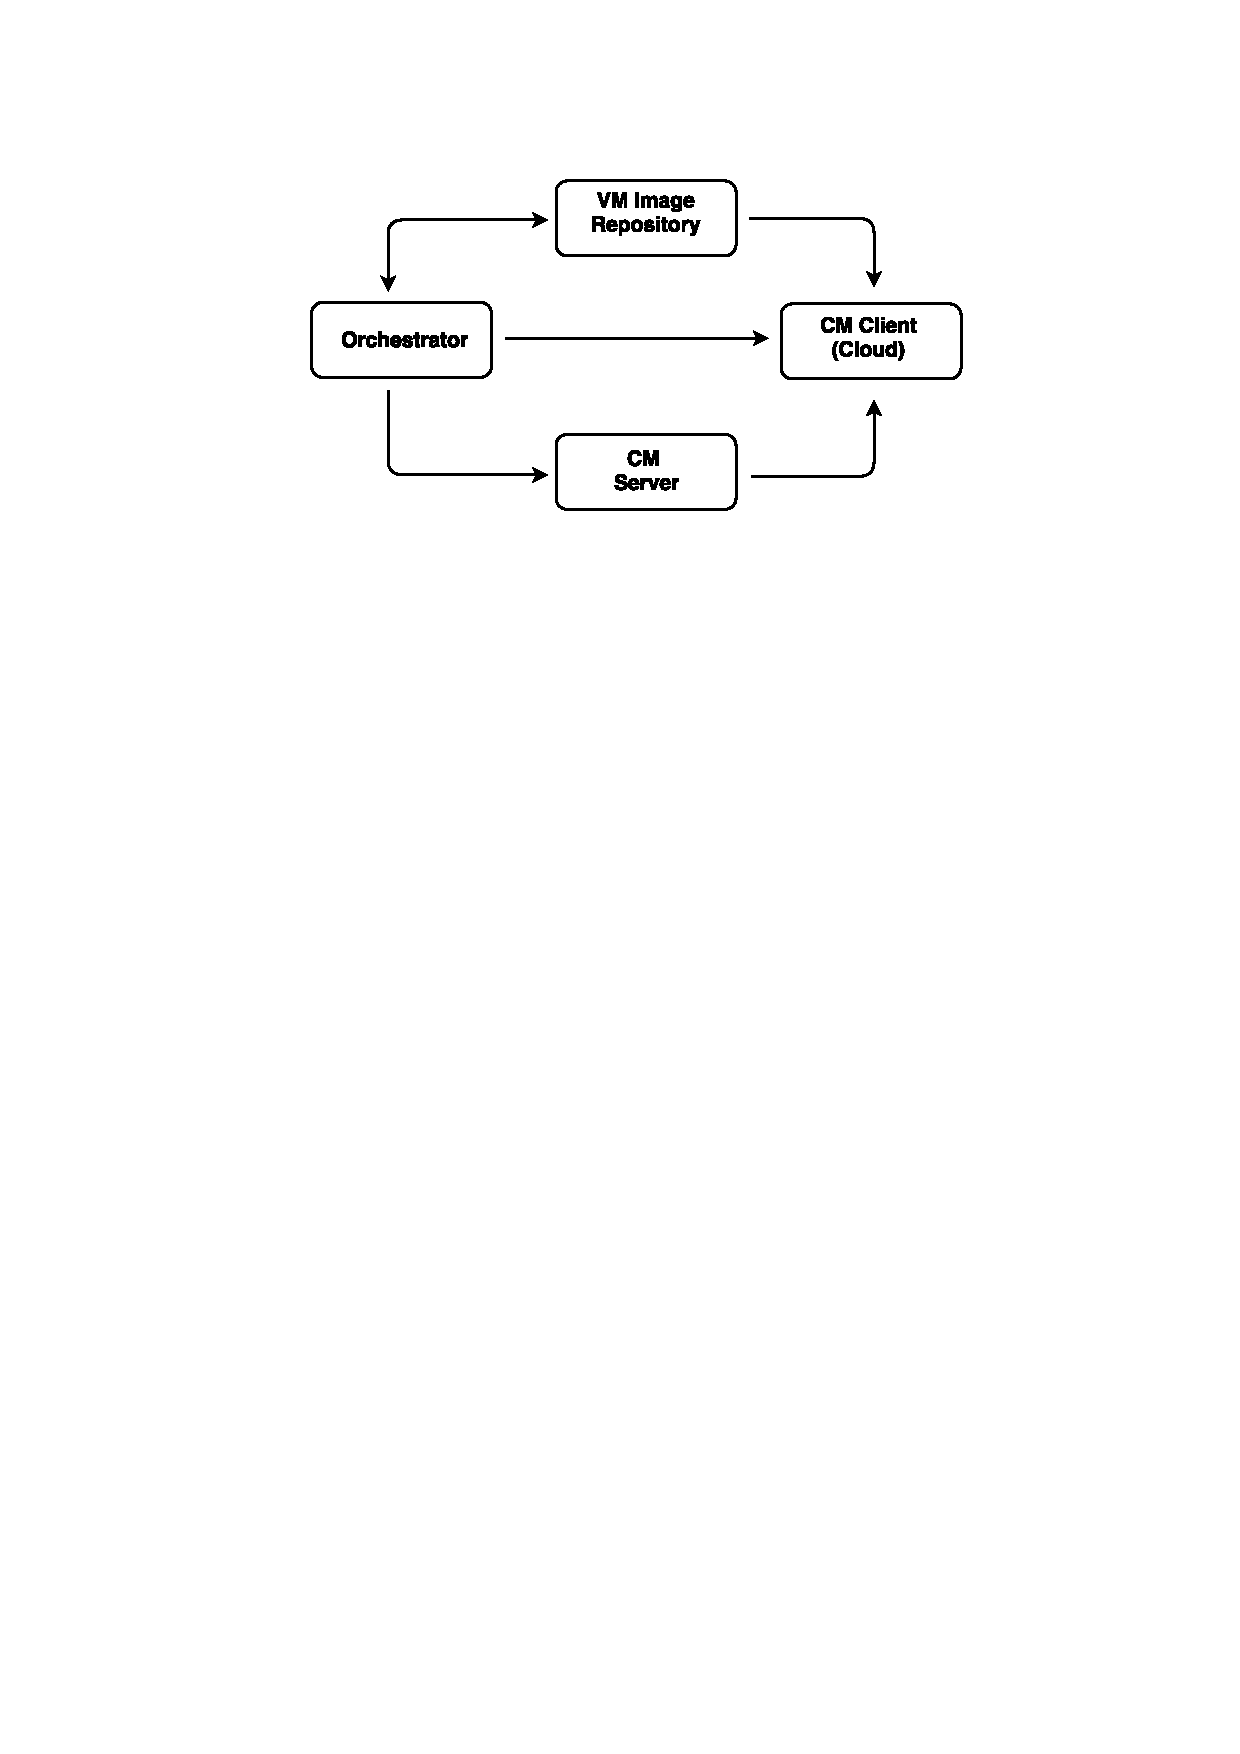
\includegraphics[width=.4\textwidth]{./figures/c4t-generic-solution.pdf}
  \caption[Provisioning mechanism conceptual architecture.]{Provisioning mechanism conceptual architecture.}
  \label{fig:provisioning_generic_architecture}
\end{figure}

In the proposed approach, the provisioning of a smart warehouse is based on provisioning policies and
software images that are defined and configured in a development environment. The provisioning policies
allow to define which components of software must be provisioned in a given instance, configure
management tasks such as to trigger a notification when a resource state changes. The software images
contains all the software components required to deploy the smart warehouse application.

After the provisioning policies were defined and configured, the Orchestrator uploads them to its respective
remote repositories (CM Server and VM Image Repository). When the provisioning request is performed -
through a configuration management interface provided by the Orchestrator - the configuration management
client (\gls{CM} Client) in the cloud server pulls the polices from the configuration management server
(\gls{CM} Server), a centralized server that is responsible to maintain a consistent state of the
provisioned nodes in the cloud. In order to enforce the polices, the \gls{CM} Client pulls the software
images from a central repository and then performs the provisioning and configuration of the software.
After provisioning the infrastructure, the CM client periodically polls the CM server in order to
determine if its current state is consistent with the most recent policy.

% Smart Place Provisioning
\subsubsection{Implementation Details}
\label{subs:impl_provisioning}
The implementation of the provisioning mechanism relies on the Chef tool. Chef provides several
features that allows to describe infrastructure as code. In the implementation of the provisioning
mechanism, the main features used were the Chef \textit{recipes}, \textit{roles} and the \textit{knife}
command-line tool\footnote{The tool uses culinary analogy in most of its concepts} .

In order to provisioning the smart warehouse software stack, we defined a set of recipes and roles that
are used by Chef to provisioning the application infrastructure. The recipes describe how the
Fosstrak software stack is provisioned in the cloud - since we are using Docker containers to
provisioning Fosstrak stack, the recipes describe how the containers must be provisioned -
and the roles allow to specify which recipes must be applied to a given node as well to
attribute responsibilities to a specific node in the provisioned infrastructure.

% Provisioning Mechanism
\paragraph{Provisioning Mechanism}
\label{par:provisioning_mechanism}
To provisioning the resources in the cloud instances we will use \textit{knife}, a command-line tool
developed by Chef that provides an interface between the local Chef repository and the Chef server.
The provisioning workflow is illustrated in Figure~\ref{fig:provisioning_tech_architecture}.

% Automatic provisioning diagram
\begin{figure}[ht!]
  \centering
  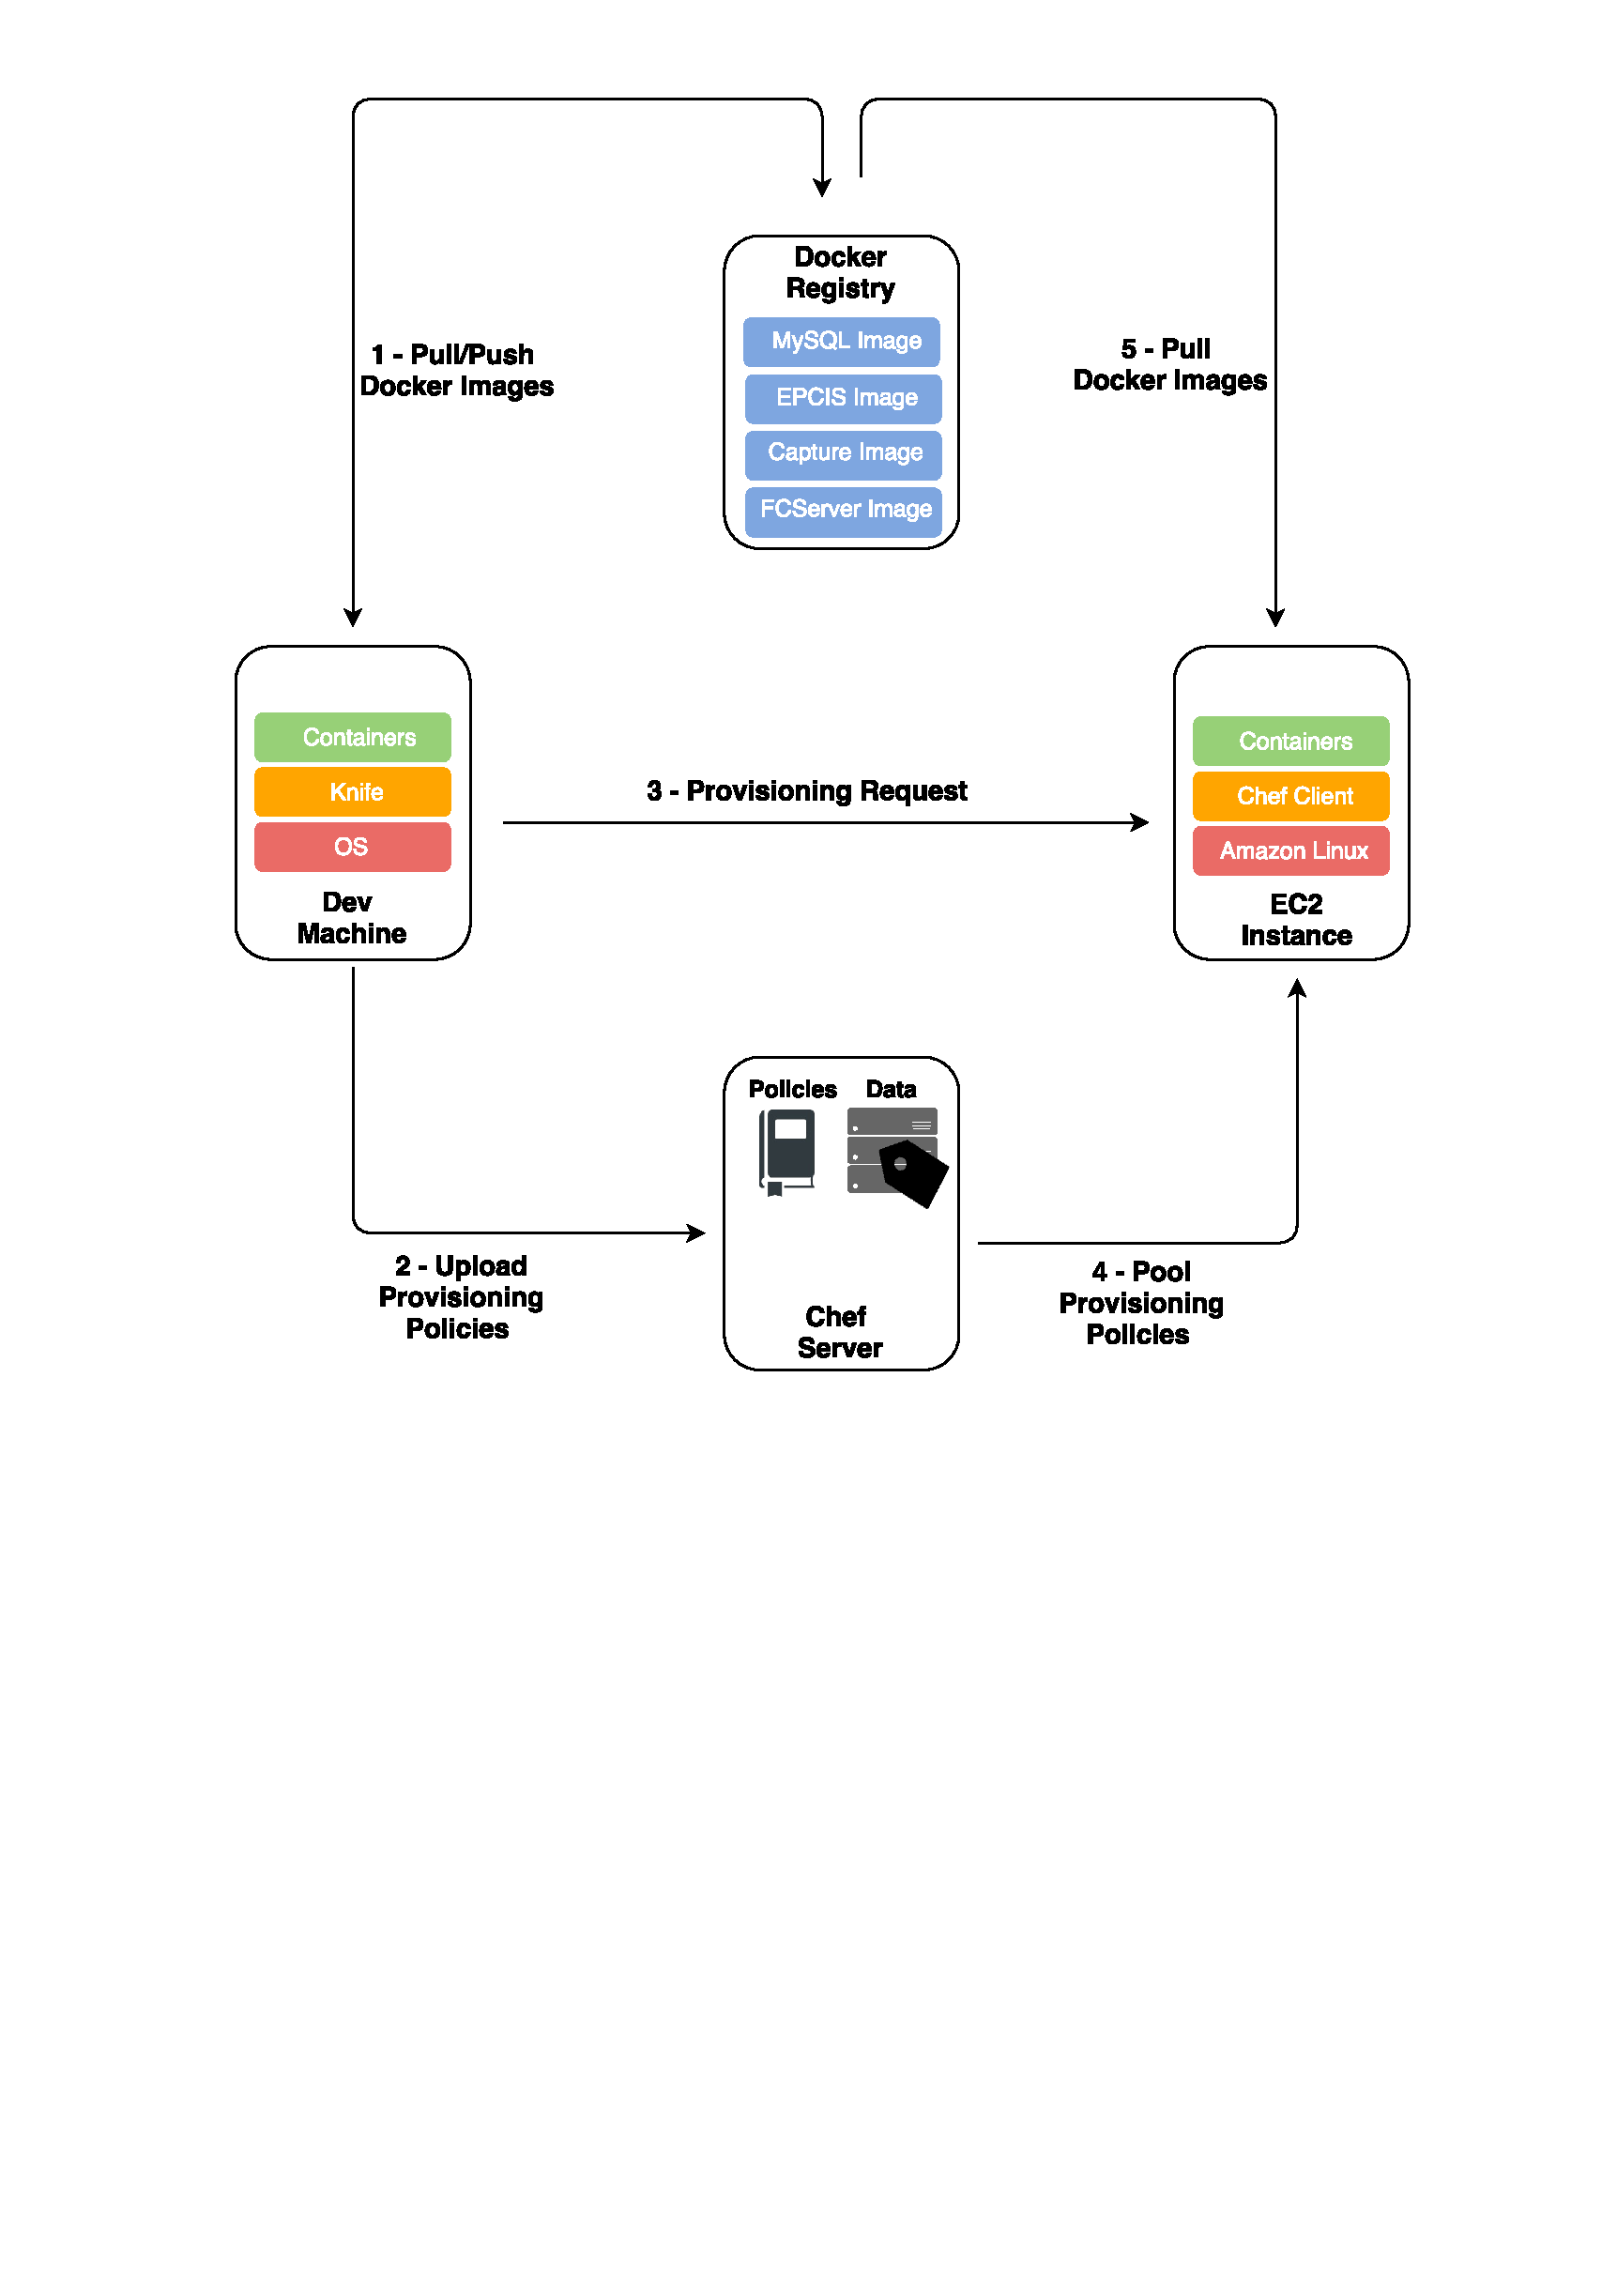
\includegraphics[width=.5\textwidth]{./figures/c4t-tech-architecture}
  \caption{Automatic provisioning mechanism architecture.}
  \label{fig:provisioning_tech_architecture}
\end{figure}

In a development environment the Docker images are built and then uploaded to the Docker Registry
repository (1). The provisioning of the cloud resources is described in the cookbooks that are uploaded
to the Chef server (2). The provisioning request (3) is performed using \textit{knife}, that allows to
describe the image type, the instance type and the policies - e.g. the \textit{role(s)} and/or \textit{recipe(s)} -
that need to be applied on each provisioned node. Then the Chef client runs the configuration policies
that are pulled from the Chef server (4). In our solution the Chef client apply the configuration recipes
that are described in the role assigned to the node. The Chef client pulls the Docker images from the
remote repository, build the containers based on those images and finally applies the configuration
that is associated to each container.

We decide to chose Chef instead of its competitors - i.e. Puppet and Ansible - for several
reasons, where the main one is \textit{knife}. Knife tool is very powerful and allow us to
interact with our entire infrastructure. Furthermore, with \textit{knife ssh} it is possible
to execute a command on a certain number of nodes in our environment. For instance, if we change
the role configuration that is assigned to a set of nodes in our infrastructure, knife allows to
update all these nodes with the most recent policy with a single command.

% Smart Warehouse Deployment
\subsection{Smart Warehouse Deployment}
\label{sub:sol_smart_warehouse_deployment}
In traditional solutions, the application is provisioned in a local infrastructure. Although such
approach guarantees that the low-latency requirements are meet, this solution comes with several
downsides - such as the low scalability, infrastructure and maintenance costs - that can be a
barrier for these applications.

Leveraging the infrastructure required to provisioning the smart warehouse application to the cloud
guarantees that the downsides of traditional solutions are solved. However, we also need to
guarantee that the latency requirements of these applications are fulfilled. The cloud and fog concepts
give us more flexibility to perform the deployment of smart warehouse applications, which allow us to
provisioning the application modules in a more distributed way. The following sections describe
the deployment approaches of smart warehouse applications based in the cloud and fog concepts.

% Cloud approach
\subsubsection{Cloud Deployment}
\label{subs:sol_cloud}
The warehouse is composed of smart objects, sensors and readers that capture the events that occurs
in the warehouse. The application middleware is provisioned in the cloud, which virtualizes the computing,
storage and network resources needed to support the application. The smart warehouse can be connected
to the cloud through a physical or wireless connection.

\paragraph{Implementation Details}
\label{par:imp_smart_warehouse_cloud}

% Cloud approach
\begin{figure}[ht!]
\centering
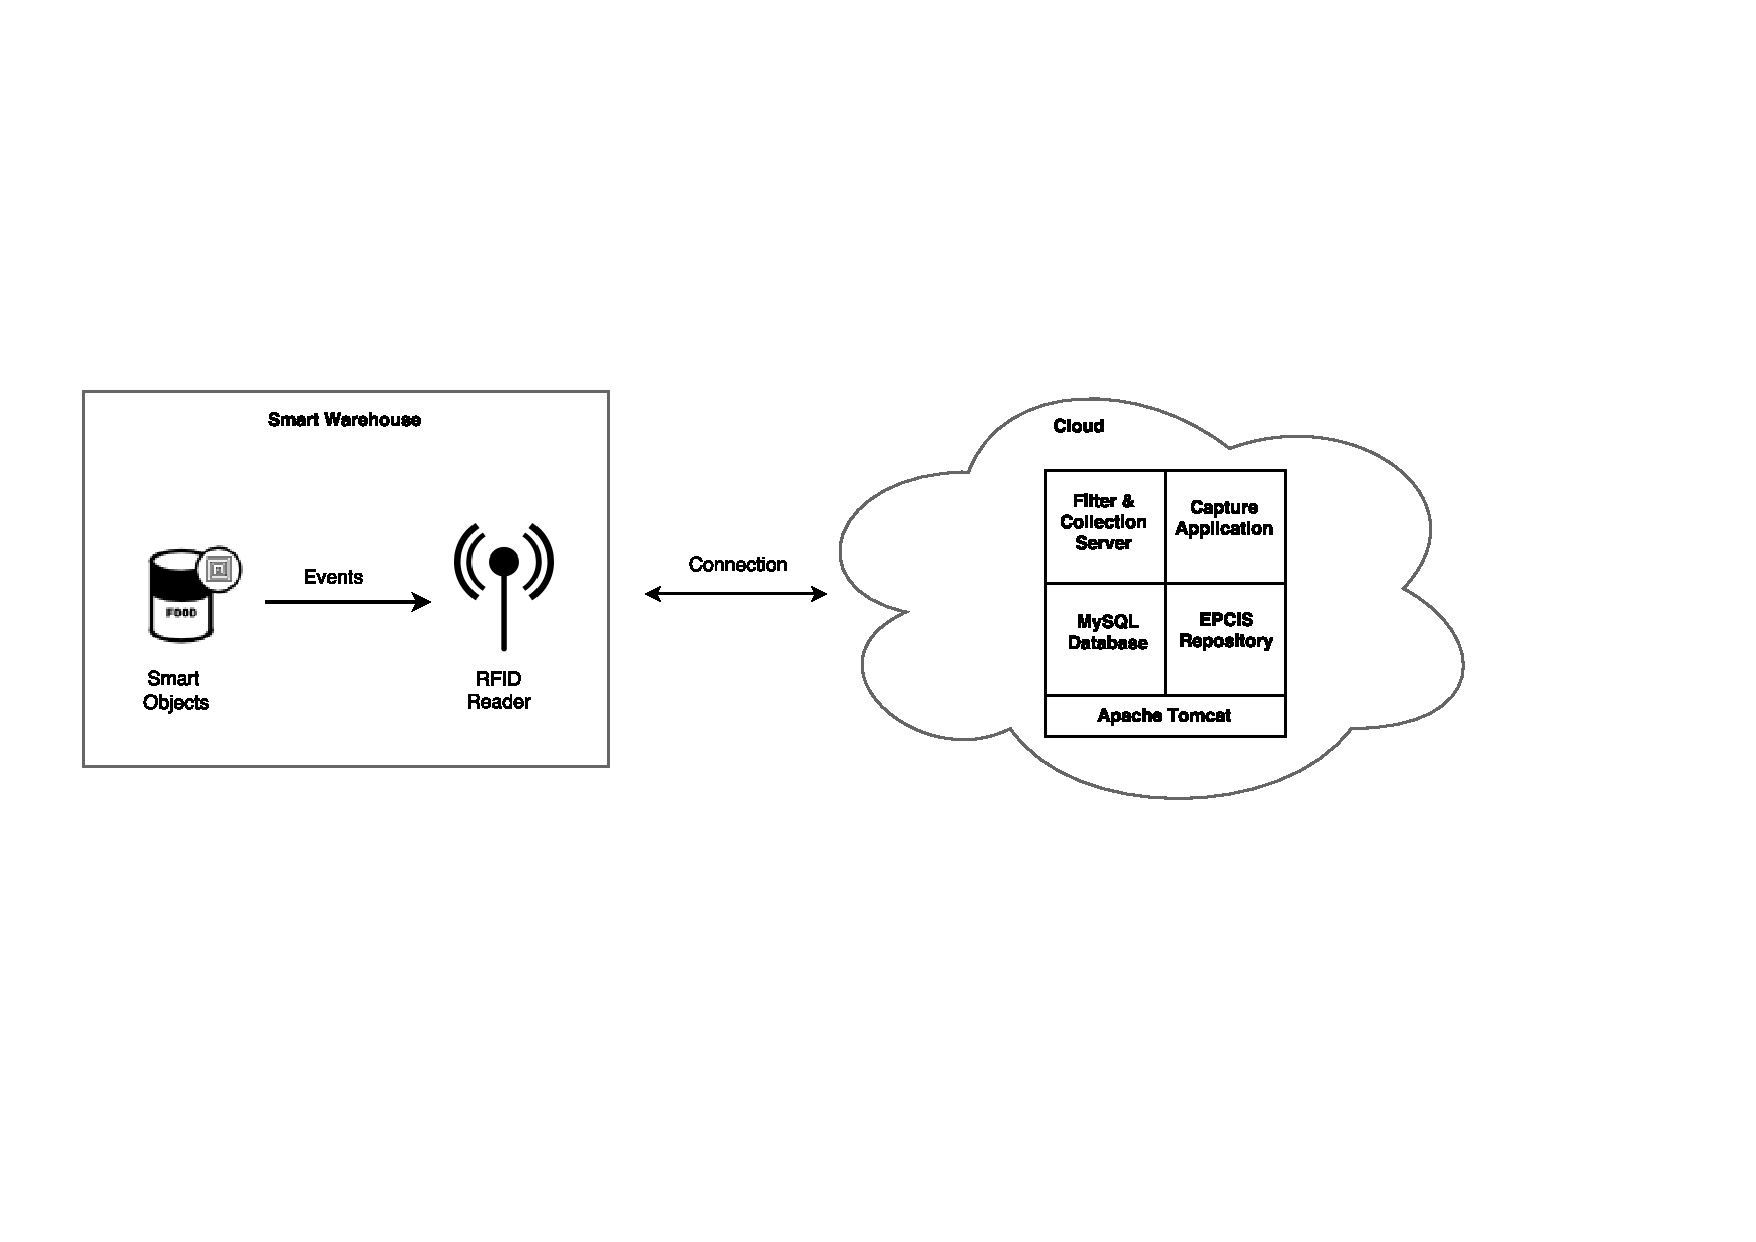
\includegraphics[width=.5\textwidth]{./figures/implementation_cloud_architecture}
\caption{Cloud deployment: smart warehouse technological architecture.}
\label{fig:implementation_cloud_architecture}
\end{figure}

The \gls{RFID} middleware is provisioned in the cloud in a single virtual machine. In the
Fosstrak implementation the \gls{FCServer}, \gls{EPCIS} repository and the Capture application
requires an Apache servlet container to deploy and run the web applications. The \gls{EPCIS}
repository is connected to a MySQL database that stores the event data. The smart warehouse can be
connected to the cloud through a physical (e.g. \gls{ADSL} or Fiber-optic) to a wireless
connection (e.g. Wi-Fi, 3G or \gls{LTE}), as illustrated in Figure~\ref{fig:implementation_cloud_architecture}.

% Fog approach
\subsubsection{Fog Deployment}
\label{subs:sol_fog}
As in the cloud-based deployment the warehouse is composed of smart objects, sensors and readers.
The proposed approach aims to extend the cloud paradigm to the edge of the network. Unlike the
cloud infrastructure, that usually is provisioned thousands of kilometers from the smart warehouse,
the fog infrastructure usually is provisioned closest to the smart warehouse network.

Regarding the application middleware, the application components are distributed across the cloud and
fog. The components responsible for storing the data during a long period of time are provisioned in
the cloud. The components responsible for performing real-time processing of the data generated in the
warehouse, and the components that filter the data that is consumed locally and must be delivered to
the cloud are provisioned in the fog. Both the smart warehouse as the fog can be connected respectively
to the fog and cloud through several types of connection, from a physical connection to a wireless
connection.

\paragraph{Implementation Details}
\label{par:imp_smart_warehouse_fog}

% Fog approach
\begin{figure}[ht!]
\centering
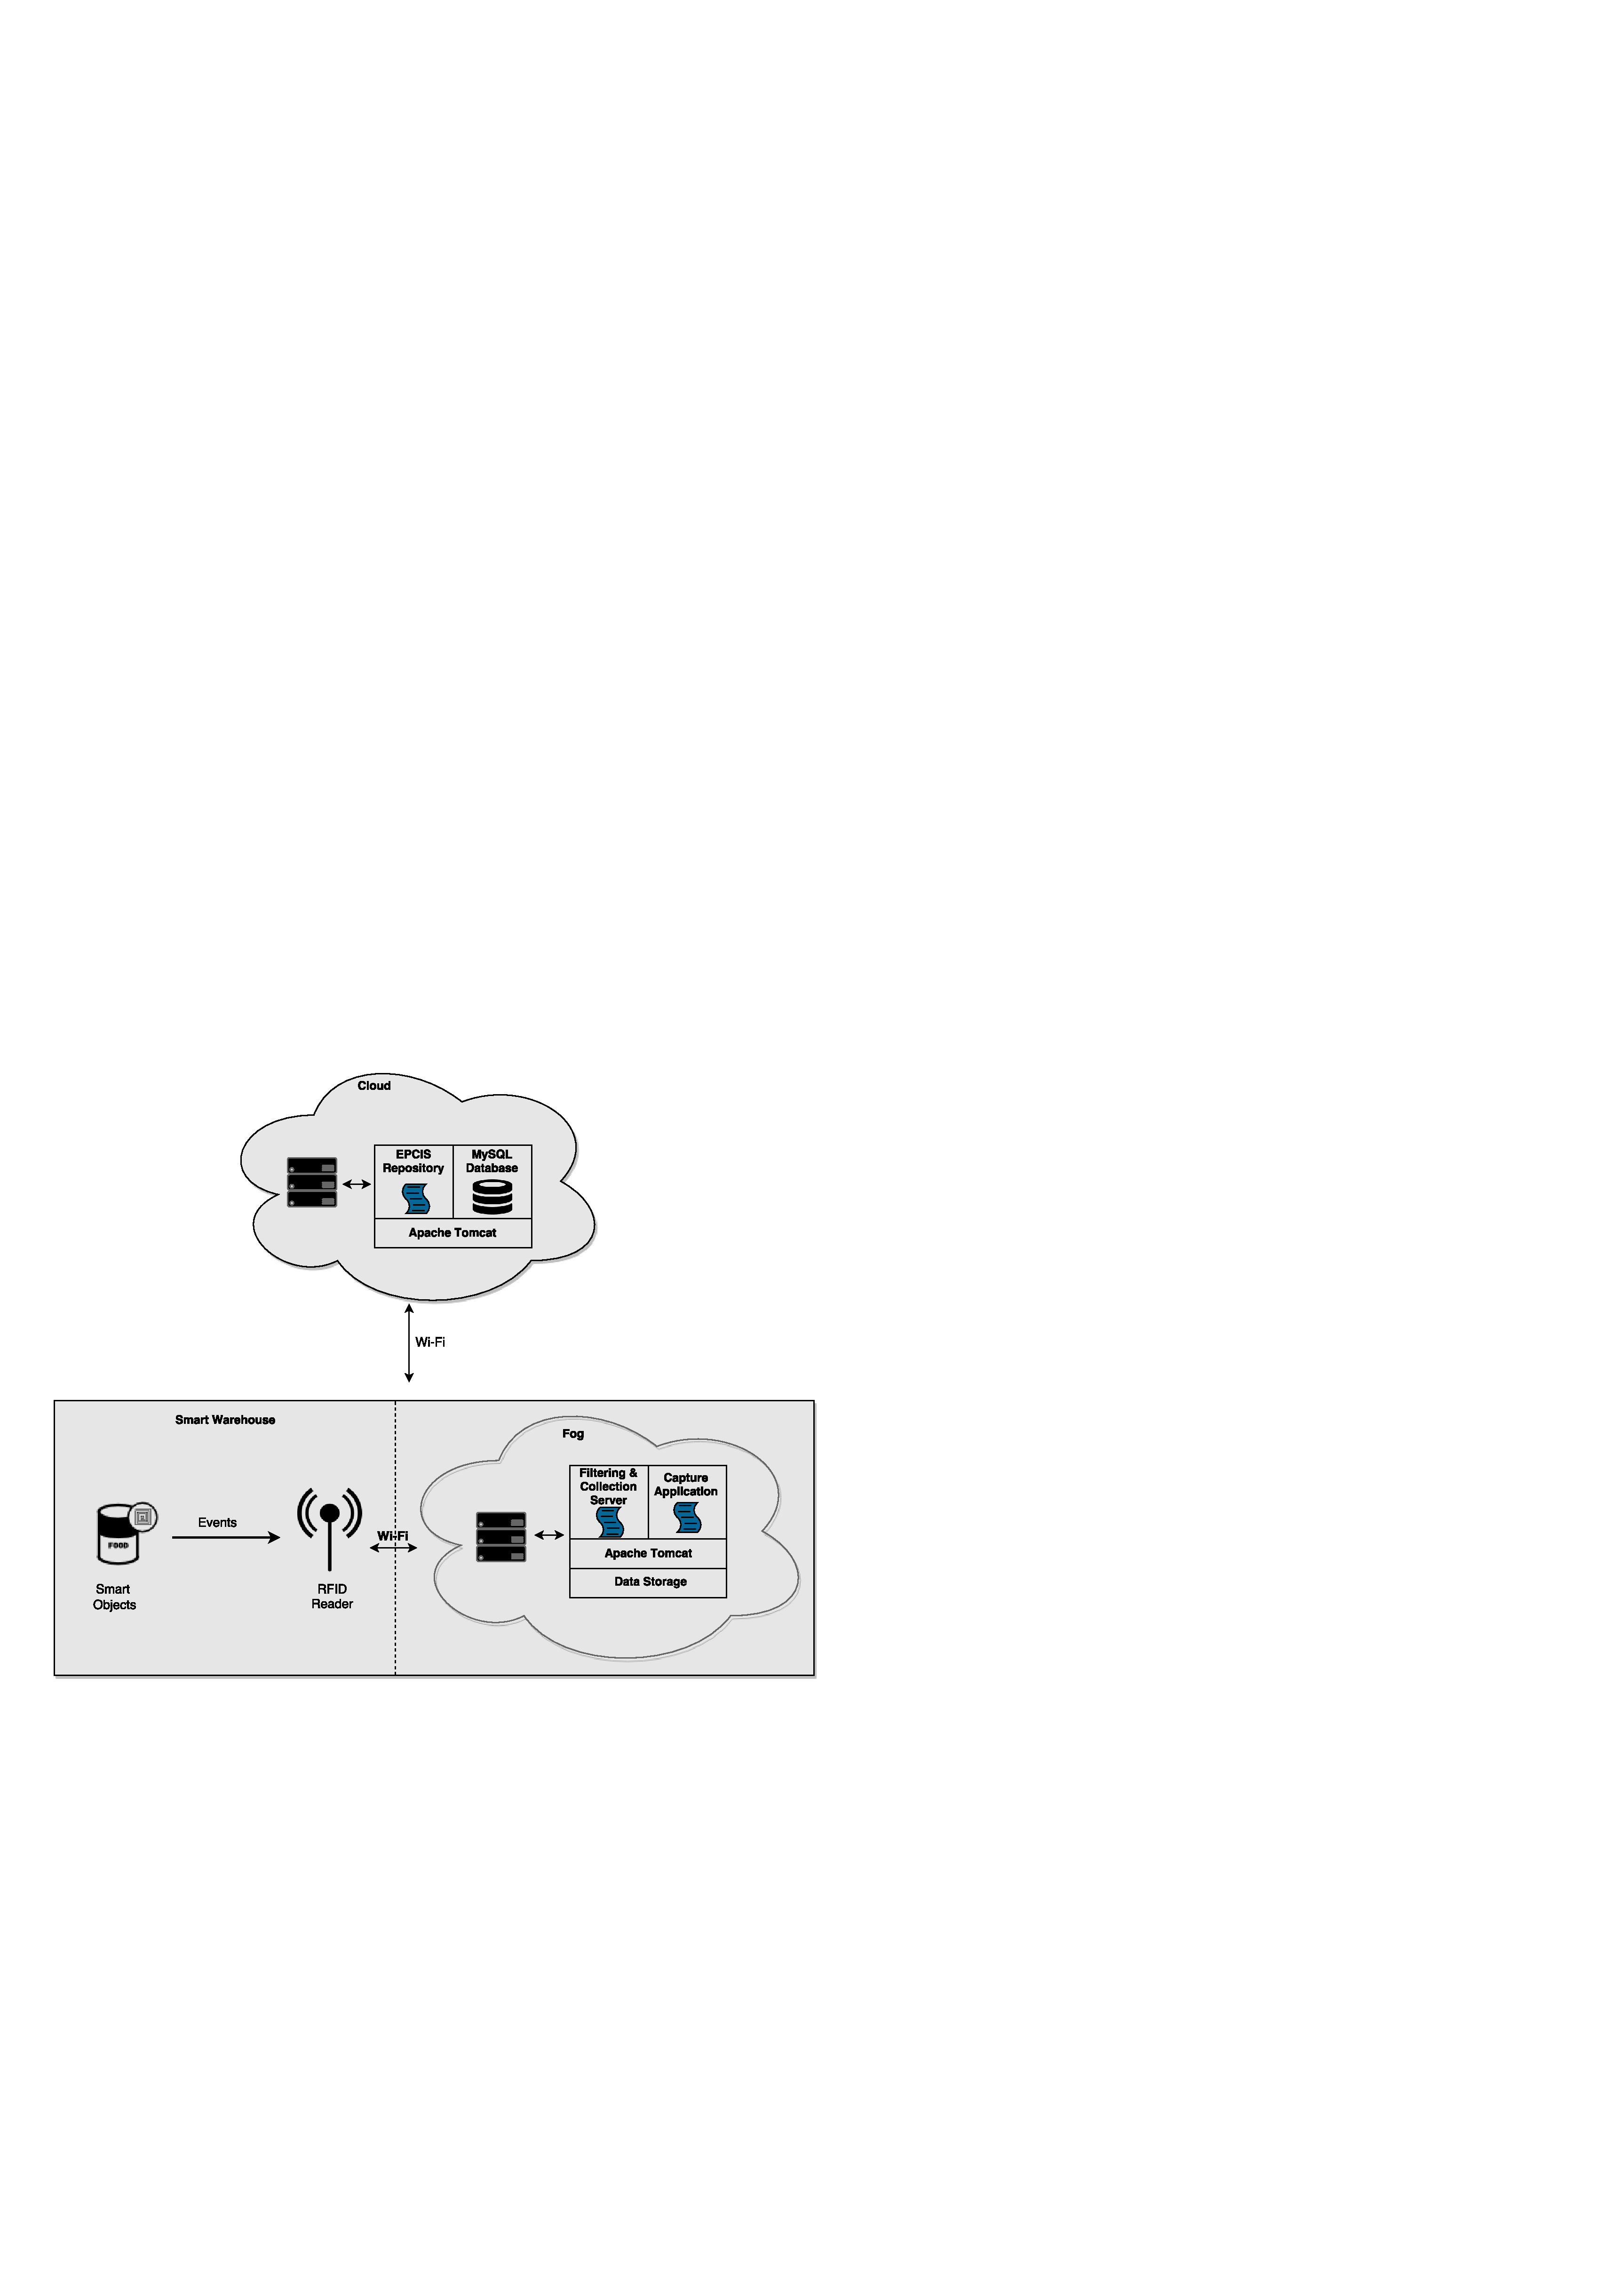
\includegraphics[width=.5\textwidth]{./figures/implementation_fog_architecture}
\caption{Fog-deployment: smart warehouse technological architecture.}
\label{fig:implementation_fog_architecture}
\end{figure}

The \gls{RFID} middleware is provisioned across the fog and the cloud. At the cloud,
all the software components are provisioned in a single \gls{VM}. The \gls{EPCIS} repository is deployed
and running on top of an Apache Tomcat servlet instance. The repository is connected to a MySQL
database, which stores the event data. In the current implementation the fog was built with a traditional
\gls{VM}. The \gls{FCServer} and the Capture application are deployed and running on top of a single
Tomcat servlet instance. The Capture application sent the events collected by the \gls{FCServer} to
the \gls{EPCIS} repository through the \textit{\gls{EPCIS} Capture Interface} - via \gls{HTTP} requests.
Both the smart warehouse as the fog can be connected respectively to the fog and cloud through several
types of connection, from a physical connection (e.g. \gls{ADSL} or Fiber-optic) to a wireless connection
(e.g. Wi-Fi, 3G or \gls{LTE}), as illustrated in Figure~\ref{fig:implementation_fog_architecture}. 
